% Autogenerated translation of EMG.md by Texpad
% To stop this file being overwritten during the typeset process, please move or remove this header

\documentclass[12pt]{book}
\usepackage{graphicx}
\usepackage{fontspec}
\usepackage[utf8]{inputenc}
\usepackage[a4paper,left=.5in,right=.5in,top=.3in,bottom=0.3in]{geometry}
\setlength\parindent{0pt}
\setlength{\parskip}{\baselineskip}
\setmainfont{Helvetica Neue}
\usepackage{hyperref}
\pagestyle{plain}
\begin{document}

\chapter*{Project 2: EMG reflex}

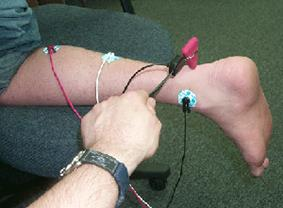
\includegraphics{project_2_EMG/EMG_diagram_2.jpeg}
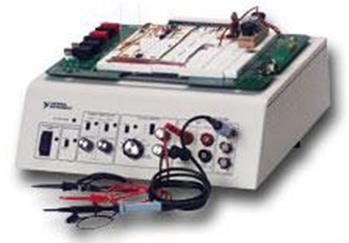
\includegraphics{project_2_EMG/EMG_diagram.jpeg}

\subsection*{Project information}

\begin{itemize}
\item \href{project_2_EMG/project_2_EMG.pdf}{Assignment description and learning objectives}
\item \href{project_2_EMG/EMG_report_DRAFT_rubric.pdf}{Report draft rubric}
\item \href{project_2_EMG/EMG_report_rubric.pdf}{Final report rubric}
\end{itemize}

\subsection*{Weekly lab exercises}

\begin{itemize}
\item Week 1 (10/17): \href{project_2_EMG/EMG_lab_1.pdf}{Lab protocol} and \href{project_2_EMG/EMG_lab_1_assignment.pdf}{in class assignment}
\item Week 2 (10/24): \href{project_2_EMG/EMG_lab_2.pdf}{Lab protocol} and \href{project_2_EMG/EMG_lab_2_assignment.pdf}{in class assignment}
\item Week 3 (10/31): \href{project_2_EMG/EMG_lab_3.pdf}{Lab protocol} and \href{project_2_EMG/EMG_lab_3_assignment.pdf}{in class assignment}
\item Week 4 (11/07): \href{project_2_EMG/EMG_lab_4.pdf}{Lab protocol} and \href{project_2_EMG/EMG_lab_4_assignment.pdf}{in class assignment}
\item Week 5 (11/14): \href{project_2_EMG/EMG_lab_5.pdf}{Lab protocol}
\item Week 6 (11/28): \textbf{Project demos and report due!}
\end{itemize}

\end{document}
